\subsection{Multi-source Even Data Injection}
\newpage
\Fig{how_voronoi} \cite{grima2013computational} provides a torus Voronoi method, which extends the original domain to $8$ copy and calculate the Voronoi Diagram as planner algorithm \cite{fortune1987sweepline}.  Then the corner part is the torus Voronoi diagram.

\begin{figure}[!ht]
\centering
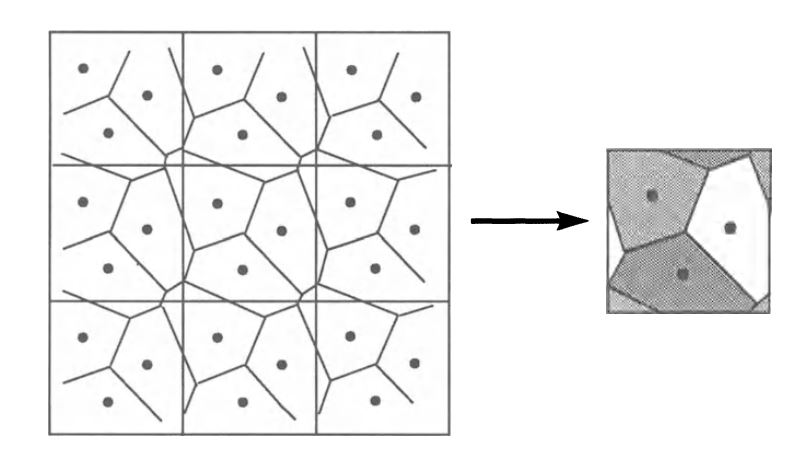
\includegraphics[width=1\columnwidth]{figure/how_voronoi.JPG}
\caption{How to calculate torus Voronoi Diagram}
\label{fig:how_voronoi}
\end{figure}

\begin{figure}[!ht]
\centering
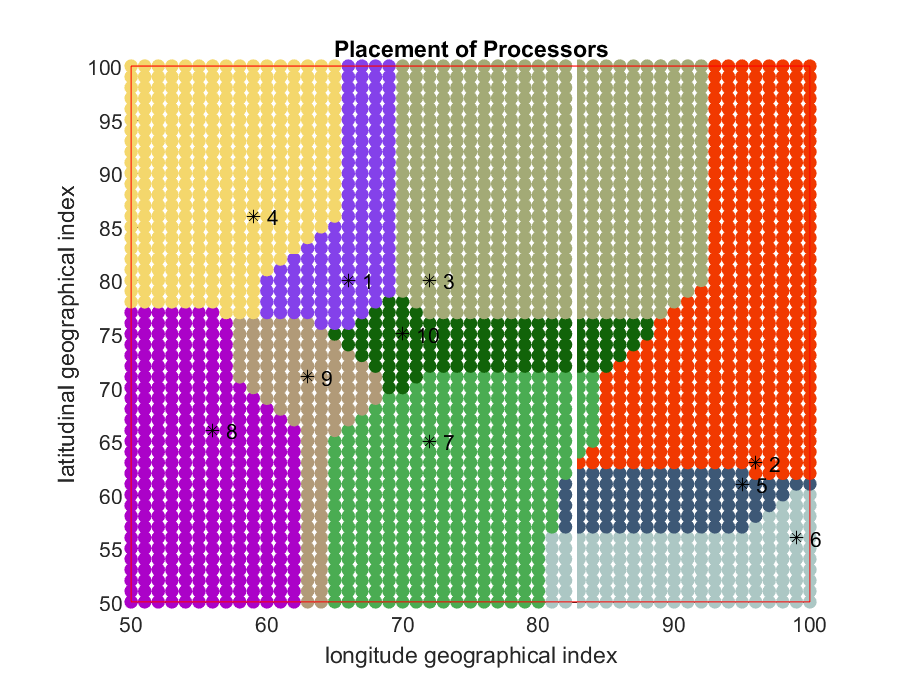
\includegraphics[width=1\columnwidth]{figure/t_1.eps}
\caption{Initial Voronoi Digram}
\label{fig:t_1}
\end{figure}

\begin{figure}[!ht]
\centering
\includegraphics[width=1\columnwidth]{figure/t_voronoi.eps}
\caption{Torus Voronoi Diagram}
\label{fig:t_voronoi}
\end{figure}

\begin{figure}[!ht]
\centering
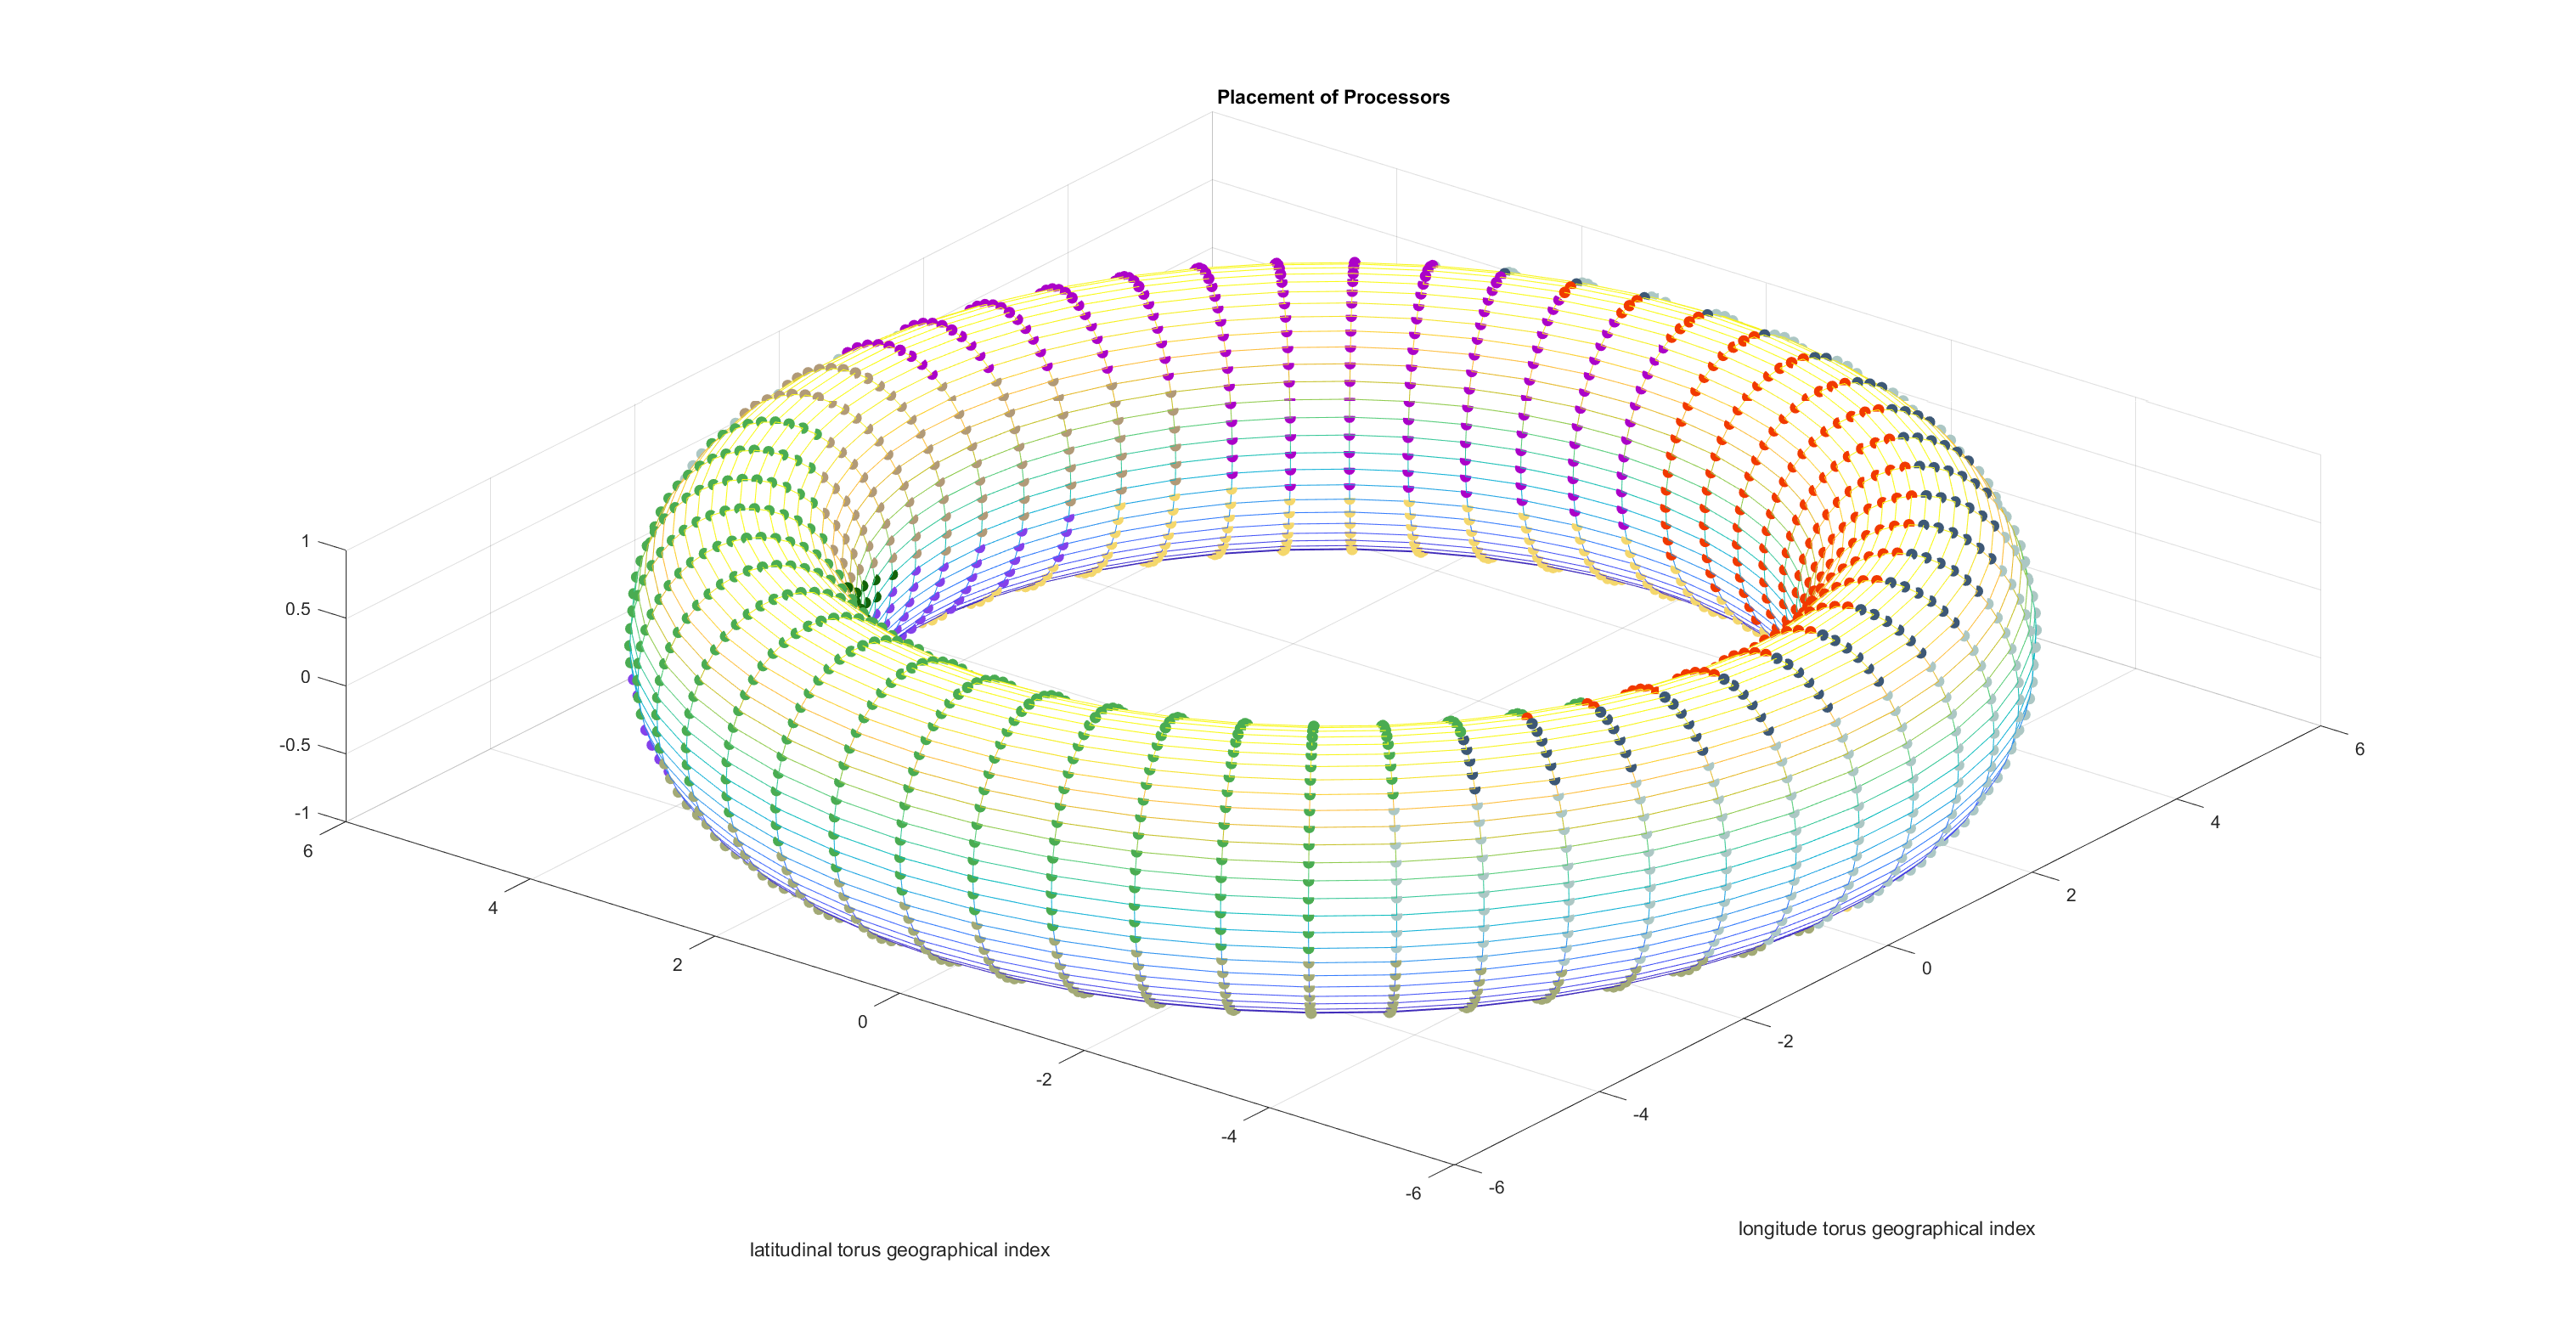
\includegraphics[width=1\columnwidth]{figure/t_voronoi_torus.eps}
\caption{Voronoi Diagram Casting to the torus model}
\label{fig:t_voronoi_torus}
\end{figure}

\begin{figure}[!ht]
\centering
\includegraphics[width=1\columnwidth]{figure/t_voronoi_speedup.eps}
\caption{Voronoi Diagram Casting to the torus model}
\label{fig:t_voronoi_torus}
\end{figure}
\newpage

In the reduced model, reduced toroidal Voronoi diagram save $27\%$ processors hit the same processing capacity.  The ratio of original method is about $\frac{490}{98} = 5$, after the reduced action, the ratio is $\frac{290}{98} \approx 2.96 $ . That is the reduced heuristic algorithm obtaining more balanced computation capacity distribution.

\begin{figure}[!ht]
\centering
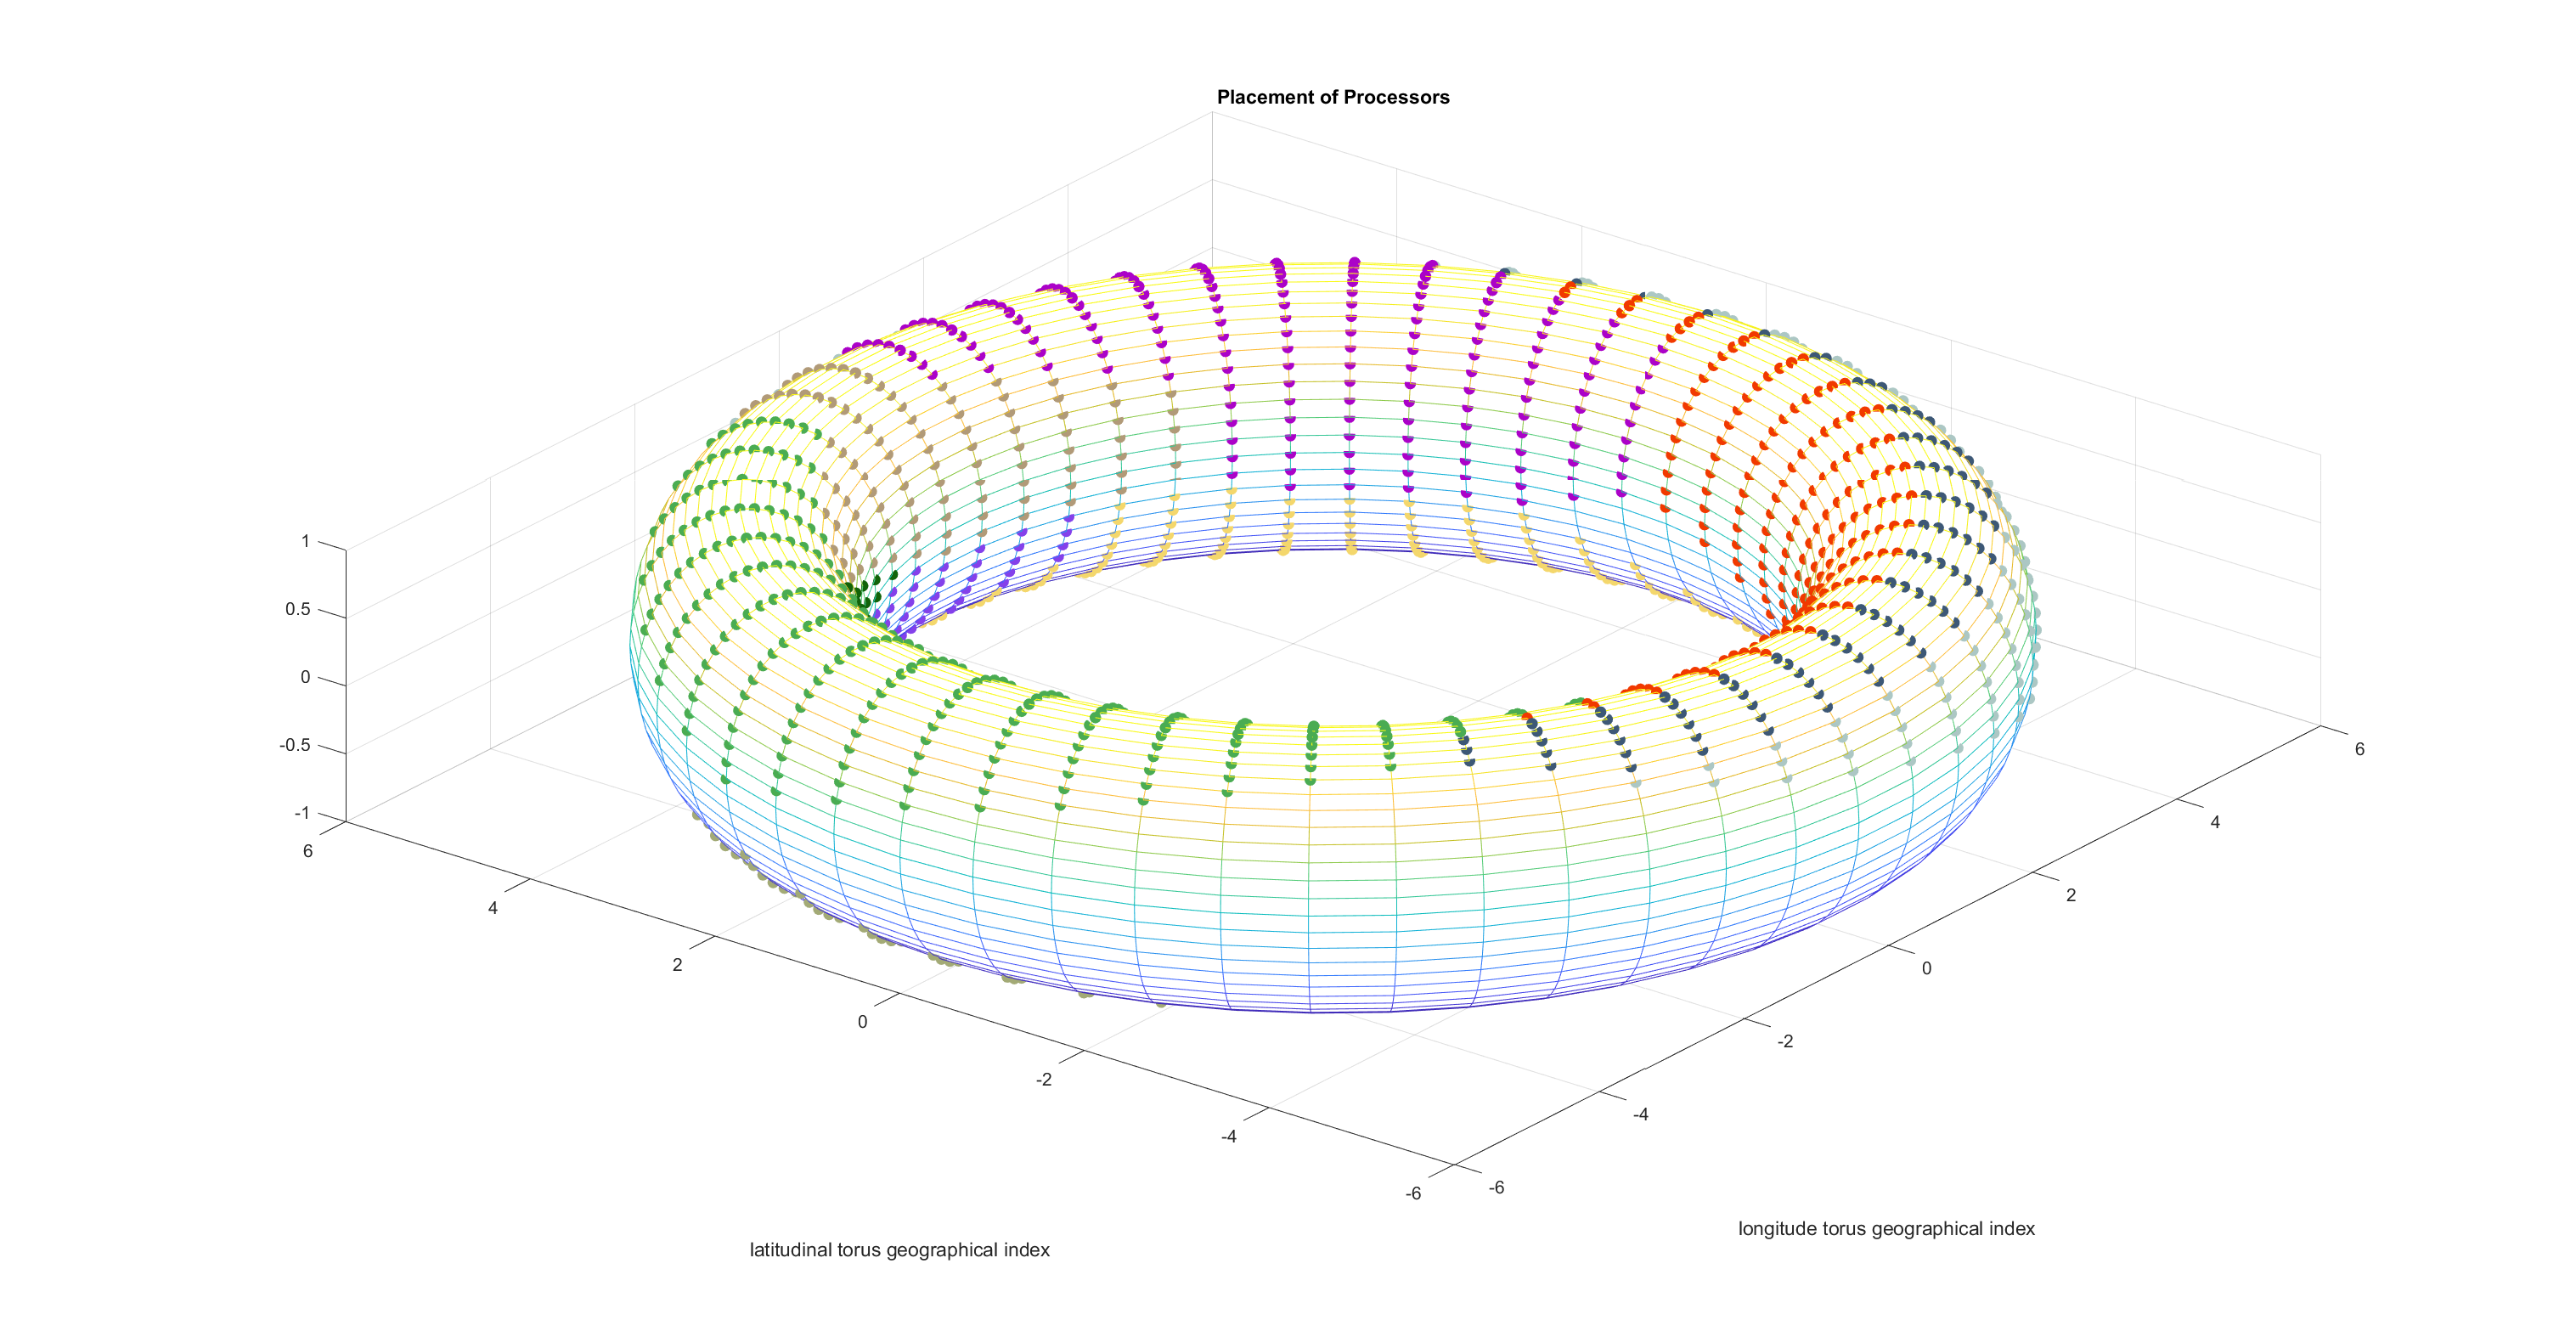
\includegraphics[width=1\columnwidth]{figure/t_voronoi_torus_save.eps}
\caption{Torus Reduced Voronoi Diagram Casting to the Torus Model}
\label{fig:t_voronoi}
\end{figure}

\begin{figure}[!ht]
\centering
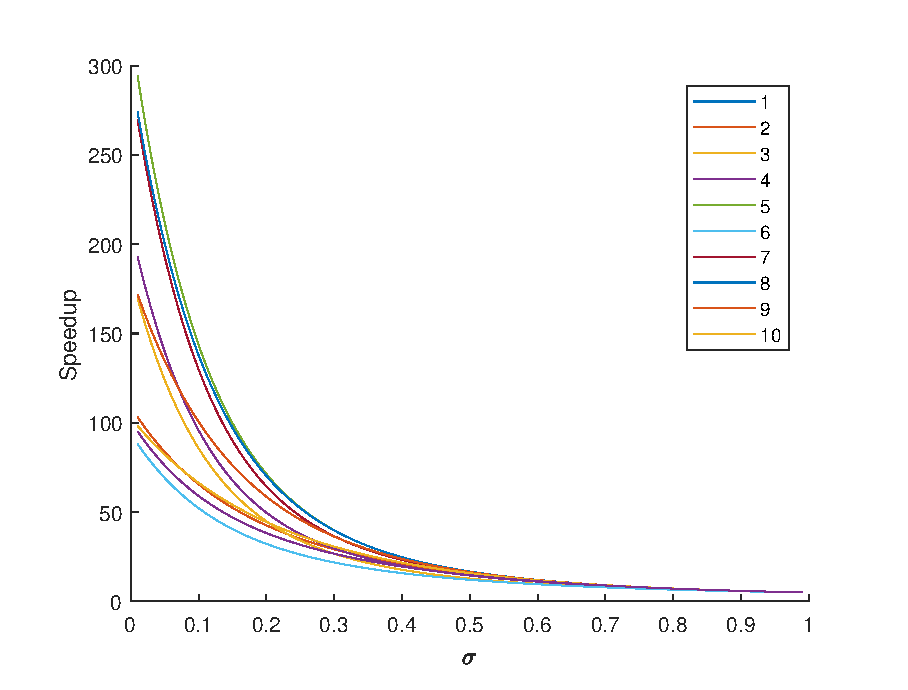
\includegraphics[width=1\columnwidth]{figure/t_voronoi_speedup_save.eps}
\caption{Torus Reduced Voronoi Diagram}
\label{fig:t_voronoi}
\end{figure}

